\section*{Chapter 8}

\subsection*{Exercise 8.1}
The nonplanning method looks particularly poor in Figure 8.3 because it is
a one-step method; a method using multi-step bootstrapping would do better. Do you
think one of the multi-step bootstrapping methods from Chapter 7 could do as well as
the Dyna method? Explain why or why not.

\subsubsection*{Solution:}
While multi-step bootstrapping methods can improve over one-step methods and perform
reasonably well, they are unlikely to match the performance of the Dyna method. The key
difference lies in the use of a model: Dyna exploits the additional simulated experience
generated by the model to accelerate learning, something that multi-step methods cannot
achieve.

\subsection*{Exercise 8.2}
Why did the Dyna agent with exploration bonus, Dyna-Q+, perform
better in the first phase as well as in the second phase of the blocking and shortcut
experiments?

\subsubsection*{Solution:}

In Phase 1, the Dyna-Q+ agent performed better because its exploration bonus encouraged
it to visit less-explored state-action pairs. The Dyna-Q agent did not have this,
so it was trying to search for the optimal path randomly.

\subsection*{Exercise 8.3}
Careful inspection of Figure 8.5 reveals that the difference between Dyna-Q+
and Dyna-Q narrowed slightly over the first part of the experiment. What is the reason
for this?

\subsubsection*{Solution:}
The exploration term in Dyna-Q+ is bigger than the exploration term in Dyna-Q, so it takes
suboptimal actions more often, consequently bringing the slope of the cumulative reward down.

\subsection*{Exercise 8.4 (programming)}
The exploration bonus described above actually changes
the estimated values of states and actions. Is this necessary? Suppose the bonus $\kappa \sqrt{\tau}$
was used not in updates, but solely in action selection. That is, suppose the action
selected was always that for which $Q(S t, a) + \kappa \sqrt{\tau(S_t, a)}$ was maximal. Carry out a
gridworld experiment that tests and illustrates the strengths and weaknesses of this
alternate approach. 

\subsubsection*{Solution:}
See the notebook.

\begin{figure}[H]
    \centering
    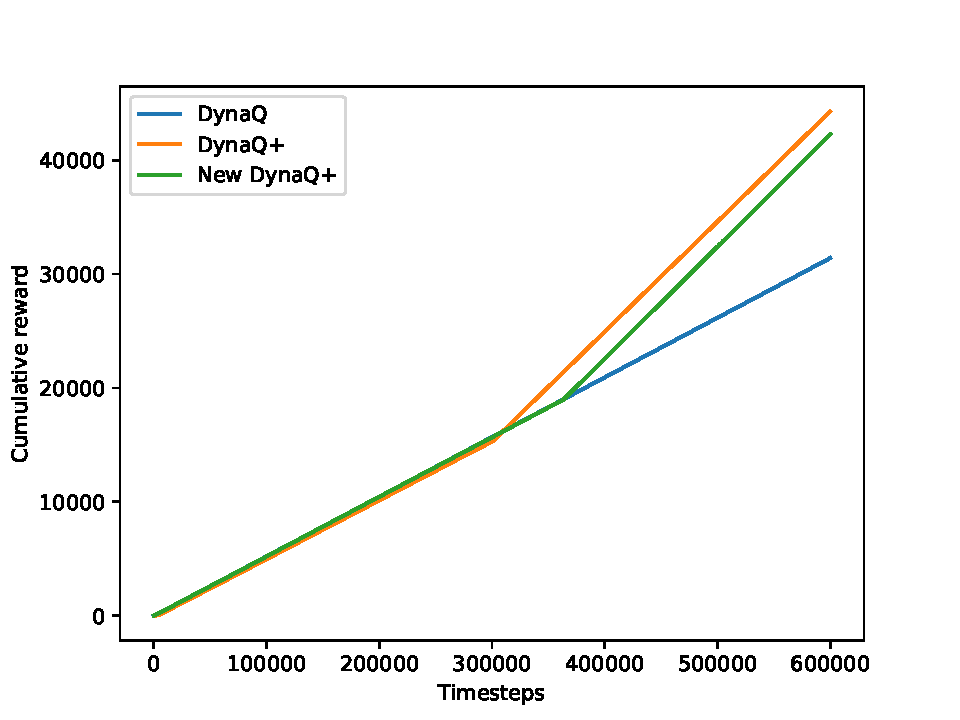
\includegraphics[width=0.8\textwidth]{chapters_latex/figures/ex_08_04.pdf}
    \captionsetup{labelformat=empty}
\end{figure}

There seems to be no significant difference between the two methods, in this case, but this may be just a coincidence. If the agent is at the shorcut location, and doesn't choose the \textit{up} action, then we have to wait again for the agent to go there again, which may take a lot of time.

\subsection*{Exercise 8.5}
How might the tabular Dyna-Q algorithm shown on page 164 be modified
to handle stochastic environments? How might this modification perform poorly on
changing environments such as considered in this section? How could the algorithm be
modified to handle stochastic environments $\textit{and}$ changing environments? 

\subsubsection*{Solution:}

We could save all the \textit{next state} and \textit{reward} pairs, and then sample from them when updating the Q-values. This would perform poorly on changing environments because the agent would be updating its Q-values with outdated information.

To handle both stochastic and changing environments, we could give more weight to the most recent experiences, and less weight to the older ones. This way, the agent would be able to adapt to the changes in the environment, and even forget about the old experiences if they are not relevant anymore.

\subsection*{Exercise 8.6}
The analysis above assumed that all of the \textit{b} possible next states were
equally likely to occur. Suppose instead that the distribution was highly skewed, that
some of the b states were much more likely to occur than most. Would this strengthen or
weaken the case for sample updates over expected updates? Support your answer. 

\subsubsection*{Solution:}
A skewed distribution strengthens the case for sample updates because they naturally focus on the most likely transitions, improving computational efficiency. However, if rare transitions are important, expected updates are better as they account for all possible outcomes. Thus, the preference depends on the importance of rare events in the problem.

\subsection*{Exercise 8.7}
Some of the graphs in Figure 8.8 seem to be scalloped in their early portions,
particularly the upper graph for $b = 1$ and the uniform distribution. Why do you think
this is? What aspects of the data shown support your hypothesis? 

\subsubsection*{Solution:}

The scalloped pattern arises because, for $b=1$ and the uniform distribution, value estimates improve significantly when new states are encountered for the first time. This creates periodic jumps in learning, as updates depend entirely on the order of state visits. Over time, as all states are visited and value estimates stabilize, the pattern smooths out.

\subsection*{Exercise 8.8 (programming)}
Replicate the experiment whose results are shown in the
lower part of Figure 8.8, then try the same experiment but with b = 3. Discuss the
meaning of your results.

\subsubsection*{Solution:}
See the notebook.

\begin{figure}[H]
    \centering
    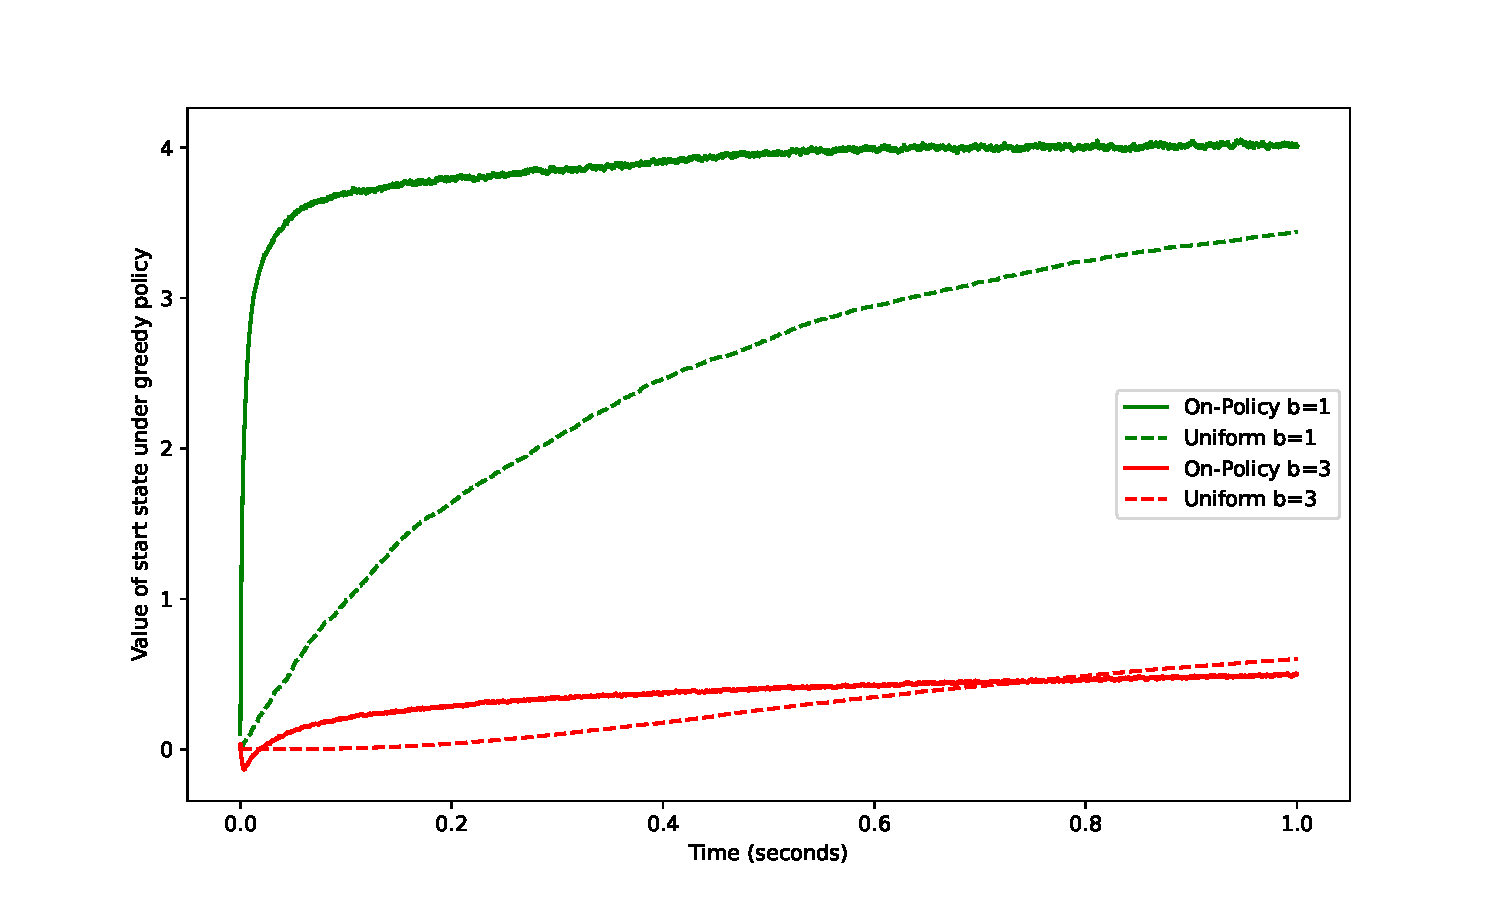
\includegraphics[width=0.9\textwidth]{chapters_latex/figures/ex_08_08.pdf}
    \captionsetup{labelformat=empty}
\end{figure}

The results discussed in the book can be seen: "The effect was stronger, and the initial period of faster planning was longer, at smaller branching factors. In other experiments, we found that these effects also became stronger as the number of states increased".